 \documentclass[12pt]{amsart}
% packages
\usepackage{graphicx}
\usepackage{setspace}
\usepackage{amssymb,amsmath,amsthm,amsfonts,amscd}
\usepackage{hyperref}
\usepackage{color}
\usepackage{booktabs}
\usepackage{tabularx}
\usepackage{enumitem}
\usepackage[retainorgcmds]{IEEEtrantools}
\usepackage[notref,notcite,final]{showkeys}
\usepackage[final]{pdfpages}
\usepackage{fancyhdr}
\usepackage{upgreek}
\usepackage{multicol}

\usepackage{fancyvrb}
\usepackage{listings}
% set margin as 0.75in
\usepackage[margin=0.75in]{geometry}

% tikz-related settings
\usepackage{tikz}
\usepackage{tikz-cd}
\usetikzlibrary{cd}

% theorem environments with italic font
\newtheorem{thm}{Theorem}[section]
\newtheorem*{thm*}{Theorem}
\newtheorem{lemma}[thm]{Lemma}
\newtheorem{prop}[thm]{Proposition}
\newtheorem{claim}[thm]{Claim}
\newtheorem{corollary}[thm]{Corollary}
\newtheorem{conjecture}[thm]{Conjecture}
\newtheorem{question}[thm]{Question}
\newtheorem{procedure}[thm]{Procedure}
\newtheorem{assumption}[thm]{Assumption}

% theorem environments with roman font (use lower-case version in body
% of text, e.g., \begin{example} rather than \begin{Example})
\newtheorem{Definition}[thm]{Definition}
\newenvironment{definition}
{\begin{Definition}\rm}{\end{Definition}}
\newtheorem{Example}[thm]{Example}
\newenvironment{example}
{\begin{Example}\rm}{\end{Example}}

\theoremstyle{definition}
\newtheorem{remark}[thm]{\textbf{Remark}}

% special sets
\newcommand{\A}{\mathbb{A}}
\newcommand{\C}{\mathbb{C}}
\newcommand{\F}{\mathbb{F}}
\newcommand{\N}{\mathbb{N}}
\newcommand{\Q}{\mathbb{Q}}
\newcommand{\R}{\mathbb{R}}
\newcommand{\Z}{\mathbb{Z}}
\newcommand{\cals}{\mathcal{S}}
\newcommand{\ZZ}{\mathbb{Z}_{\ge 0}}
\newcommand{\cala}{\mathcal{A}}
\newcommand{\calb}{\mathcal{B}}
\newcommand{\cald}{\mathcal{D}}
\newcommand{\calh}{\mathcal{H}}
\newcommand{\call}{\mathcal{L}}
\newcommand{\calr}{\mathcal{R}}
\newcommand{\la}{\mathbf{a}}
\newcommand{\lgl}{\mathfrak{gl}}
\newcommand{\lsl}{\mathfrak{sl}}
\newcommand{\lieg}{\mathfrak{g}}

% math operators
\DeclareMathOperator{\kernel}{\mathrm{ker}}
\DeclareMathOperator{\image}{\mathrm{im}}
\DeclareMathOperator{\rad}{\mathrm{rad}}
\DeclareMathOperator{\id}{\mathrm{id}}
\DeclareMathOperator{\hum}{[\mathrm{Hum}]}
\DeclareMathOperator{\eh}{[\mathrm{EH}]}
\DeclareMathOperator{\lcm}{\mathrm{lcm}}
\DeclareMathOperator{\Aut}{\mathrm{Aut}}
\DeclareMathOperator{\Inn}{\mathrm{Inn}}
\DeclareMathOperator{\Out}{\mathrm{Out}}
\DeclareMathOperator{\Gal}{\mathrm{Gal}}


% frequently used shorthands
\newcommand{\ra}{\rightarrow}
\newcommand{\se}{\subseteq}
\newcommand{\ip}[1]{\langle#1\rangle}
\newcommand{\dual}{^*}
\newcommand{\inverse}{^{-1}}
\newcommand{\norm}[2]{\|#1\|_{#2}}
\newcommand{\abs}[1]{\lvert #1 \rvert}
\newcommand{\Abs}[1]{\bigg| #1 \bigg|}
\newcommand\bm[1]{\begin{bmatrix}#1\end{bmatrix}}
\newcommand{\op}{\text{op}}

% nicer looking empty set
\let\oldemptyset\emptyset
\let\emptyset\varnothing

\setlist[enumerate,1]{topsep=1em,leftmargin=1.8em, itemsep=0.5em, label=\textup{(}\arabic*\textup{)}}
\setlist[enumerate,2]{topsep=0.5em,leftmargin=3em, itemsep=0.3em}

%pagestyle
%\pagestyle{fancy} 

\begin{document}
\begin{center}
    \textsc{Random Walks. HW 3\\ Ian Jorquera\\ Collaboration: Tristan}
\end{center}
\vspace{1em}


\definecolor{codegreen}{rgb}{0,0.6,0}
\definecolor{codegray}{rgb}{0.5,0.5,0.5}
\definecolor{codepurple}{rgb}{0.58,0,0.82}
\definecolor{backcolour}{rgb}{1,1,1}

\lstdefinestyle{mystyle}{
    backgroundcolor=\color{backcolour},   
    commentstyle=\color{codegray},
    keywordstyle=\color{magenta},
    numberstyle=\tiny\color{codegray},
    stringstyle=\color{codegreen},
    basicstyle=\ttfamily\footnotesize,
    breakatwhitespace=false,         
    breaklines=true,                 
    captionpos=b,                    
    keepspaces=true,                 
    numbers=left,                    
    numbersep=5pt,                  
    showspaces=false,                
    showstringspaces=false,
    showtabs=false,                  
    tabsize=2
}

\lstset{style=mystyle}


\begin{itemize}
\item[(1)] We know that $\ip{n(t)}=\sum_{n=0}^\infty n\chi_n(t)$, meaning in the Laplace domain we have that $\ip{n(s)}=\sum_{n=0}^\infty n\hat{\chi}_n(s)$, by linearity of Laplace transforms. Furthermore we know that $\hat{\chi}_n(s)=\psi^n(s)\frac{1-\psi(s)}{s}$ meaning
$$\ip{n(s)}=\sum_{n=0}^\infty n\hat{\chi}_n(s)=\sum_{n=0}^\infty n\psi^n(s)\frac{1-\psi(s)}{s}=\frac{1-\psi(s)}{s}\sum_{n=0}^\infty n\psi^n(s)$$
Notice that this sum is a Arithmetico-geometric series(source: \href{https://en.wikipedia.org/wiki/Arithmetico-geometric_sequence}{here}) meaning we know that $\sum_{n=0}^\infty n\psi^n(s)=\frac{\psi(s)}{\left(1-\psi(s)\right)^2}$ for $0<\psi(s)<1$ and so we have that
$$\ip{n(s)}=\frac{1-\psi(s)}{s}\frac{\psi(s)}{\left(1-\psi(s)\right)^2}=\frac{\psi(s)}{s(1-\psi(s))}$$\\

\item[(2)]
Assume that $\psi(t)=A(t\ln^\beta t)^{-1}$ with $\beta>1$ and $A$ some constant.
\begin{enumerate}[label=(\alph*)]
    \item Now consider the survival probability $$\phi(t)=\int_{t}^{\infty}\psi(t')dt'=\int_{t}^{\infty}A(t'\ln^\beta t')^{-1}dt'=\left[\frac{A\ln^{1-\beta}\left(t'\right)}{1-\beta}\right]^{\infty}_{t}$$
    Which was computed using wolfram alpha

    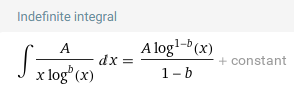
\includegraphics[scale=.8]{rw3p2int.png}

    Because $\beta>1$ we know that $\displaystyle{\lim_{t'\ra \infty} \frac{A\ln^{1-\beta}\left(t'\right)}{1-\beta}}=0$ meaning $\phi(t)=\displaystyle{\frac{-A\ln^{1-\beta}\left(t\right)}{1-\beta}}$. Notice that we can rewrite this as $\phi(t)=t^{1-1}L(t)$ such that $L(t)=\displaystyle{\frac{-A\ln^{1-\beta}\left(t\right)}{1-\beta}}$ is a slowly varying function. This means that by the Tauberian theorem we know that the Laplace transform of $\phi(t)$ is 
    $$\phi(s)=\Gamma(1)s^{-1}L(1/s)=\frac{-A\ln^{1-\beta}(1/s)}{s(1-\beta)}=\frac{A}{s(\beta-1)\ln^{\beta-1}(1/s)}$$
    Then because $\phi(s)=\frac{1-\psi(s)}{s}$ we know that $1-\psi(s)=s\phi(s)=\frac{sA}{s(\beta-1)\ln^{\beta-1}(1/s)}\propto\frac{1}{(\beta-1)\ln^{\beta-1}(1/s)}$.\\
    
    \item Consider the random walk with waiting time from part a and a step size distribution with second moment $\ip x = \sigma^2$. In this case we know that we can use the small $k$ approximation $\lambda(k) = 1-\frac{k^2\sigma^2}{2}$. And recall that 
    $$p(k,s)=\frac{1-\psi(s)}{s}\frac{1}{1-\lambda(k)\psi(s)}$$
    Which means that 
    $$p(k,s)=\frac{A}{s(\beta-1)\ln^{\beta-1}(1/s)}\frac{1}{1-(1-\frac{k^2\sigma^2}{2})\psi(s)}$$
    And now let $w(s)=1-\psi(s)=\frac{A}{(\beta-1)\ln^{\beta-1}(1/s)}$ which gives us 
    \begin{align*}
        p(k,s)&=\frac{w(s)}{s}\frac{1}{1-(1-\frac{k^2\sigma^2}{2})(1-w(s))}\\&=\frac{w(s)}{s}\frac{1}{1-(1-\frac{k^2\sigma^2}{2})(1-w(s))}\\
        &=\frac{w(s)}{s}\frac{1}{w(s)+\frac{k^2\sigma^2}{2}-\frac{k^2\sigma^2}{2}w(s)}\\
        &=\frac{w(s)}{s}\frac{1}{w(s)+\frac{k^2\sigma^2}{2}(1-w(s))}\\
        &=\frac{1}{s}\frac{1}{1+\frac{k^2\sigma^2}{2}(\frac{1}{w(s)}-1)}\\
        &=\frac{1}{s}\cdot\frac{1}{1+k^2w'(s)^2}\\
        %&=\frac{1}{s}\frac{\frac{2}{\sigma^2(\frac{1}{w(s)}-1)}}{\frac{2}{\sigma^2(\frac{1}{w(s)}-1)}+k^2}\\
        %&=\frac{1}{s}\frac{w'(s)}{w'(s)+k^2}\\
    \end{align*}
    where $w'(s)^2=\frac{\sigma^2}{2}(\frac{1}{w(s)}-1)=\frac{\sigma^2}{2A}((\beta-1)\ln^{\beta-1}(1/s)-1)$ and notice that $p(k,s)$ is slowly varying as $\frac{1}{s}\ra \infty$ because $w'(s)^2$ is slowly varying as $\frac{1}{s}\ra \infty$ witch follows from $w(s)$ being a slowly varying function as $\frac{1}{s}\ra \infty$.\\

    And so we can concluding with the Tauberian theorem that 
    $$p(k,t)=\frac{1}{1+k^2W(t)^2}$$
    For $W(t)^2=\frac{\sigma^2}{2A}((\beta-1)\ln^{\beta-1}(t)-1)$. And notice that this is the characteristic function of the Laplace distribution(source: \href{https://en.wikipedia.org/wiki/Characteristic_function_(probability_theory)}{here}) where
    $$p(x,t)=\frac{1}{2W(t)}e^{-\frac{|x|}{W(t)}}$$
    Where $W(t)=\sqrt{\frac{\sigma^2}{2A}((\beta-1)\ln^{\beta-1}(t)-1)}$\\

    \item Recall that $\ip{x^2(t)}=\ip{n(t)}\ip{\ell^2}$ and we know that 
    $$\ip{n(s)}=\frac{\psi(s)}{s(1-\psi(s))}=\frac{(\beta-1)\ln^{\beta-1}(1/s)(1-\frac{A}{s(\beta-1)\ln^{\beta-1}(1/s)})}{sA}=\frac{(\beta-1)\ln^{\beta-1}(1/s)-A}{sA}$$
    $$=\frac{(\beta-1)\ln^{\beta-1}(1/s)}{sA}-\frac{1}{s}$$
    and so by the Tauberian theorem we have that
    $$\ip{n(t)}=\frac{(\beta-1)\ln^{\beta-1}(t)}{A}-1$$
    It seems that this distribution gets the name ultra slow as the first moment for the number of steps seems to have a very small rate of change with respect $t$, an example is shown below.
    
    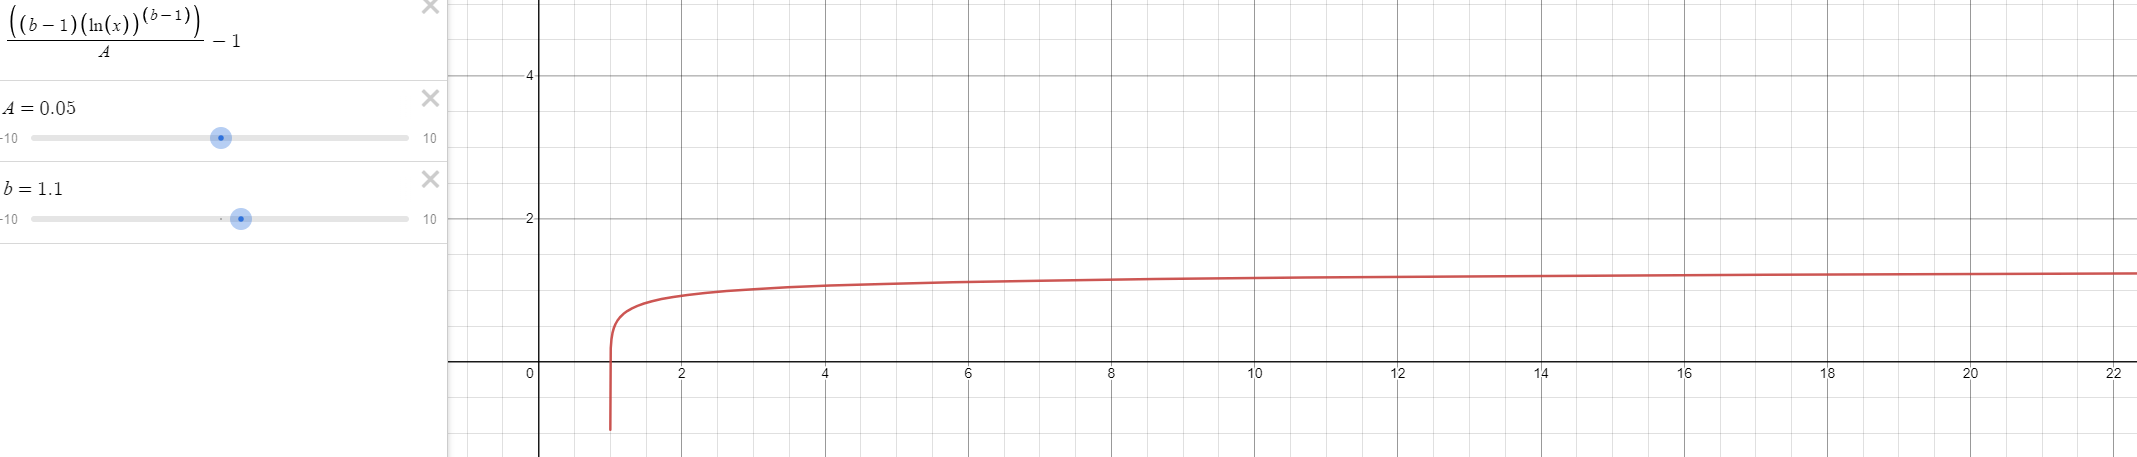
\includegraphics[scale=.45]{ultraslow.png}
    
    
    
\end{enumerate}

\item[(3)] Equation (1) refers to the second moment of a continuous time random walk after time $t$ where the random variable for $t$ has a first moment $\ip{t}$ that exists. In this equation we have that $\ip{x^2(t)}=2Kt$ where $K$ is the diffusion coefficient.

Equation (2) gives us the temporal second moment of a realization of a continuous time random walk. In this equation we are averaging the second moment over all intervals of length $t$ in a realization of length $T$.% $\ip{x^2(t)}_{T}=\frac{1}{T-t}\int_{0}^{T-t}$

Equation (3) gives the ensemble second moment of a continuous time random walk whose waiting time distribution behaves as $t^{-1-\alpha}$ for $\alpha\neq 1$. This is the case of anomalous diffusion where $K_\alpha$ is the diffusion coefficient.

Equation (4) tells us that from the independence of each step, that the second moment of a continuous time random walk is equal to the expected number of steps $\ip{n(t)}$ times the second moment of any gives step $\ip{x_1}=a^2$.\\

\item[(4)] Now we will derive equations (5) through (7).

Equation (5): Notice that becasue the the second moment is proportional to the number of steps taken we know that 
$$\ip{[x(t_2)-x(t_1)]^2}_{ens}=\ip{n(t_2)-n(t_1)}_{ens}\ip{\ell^2}=(\ip{n(t_2)}-\ip{n(t_1)}_{ens})\ip{\ell^2}=a^2(\ip{n(t_2)}-\ip{n(t_1)}_{ens})$$

Equation (6): Because the sequence of the temporal and of the ensemble average can be interchanged we have that $\ip{\ip{x^2(t)}_T}_{ens}=\ip{\ip{x^2(t)}_{ens}}_{T}$ which means 

$$\ip{\ip{x^2(t)}_{ens}}_{T}=\frac{1}{T-t}\int_{0}^{T-t}  \ip{[x(t'+t) - x(t')]^2}_{ens} dt'$$

from equations 4 we have that 

$$\frac{1}{T-t}\int_{0}^{T-t}  \ip{[x(t'+t) - x(t')]^2}_{ens} dt'=\frac{a^2}{T-t}\int_{0}^{T-t}  \ip{n(t'+t)}_{ens} - \ip{x(t')}_{ens} dt'$$

And because we are assuming that $T>>t$ we have that $T-t\approx T$. Furthermore by using $\ip{n(t)}_{ens}=At^\alpha$ we find that

$$\ip{\ip{x^2(t)}_{ens}}_{T}=\frac{a^2}{T}\int_{0}^{T} \left[ \ip{n(t'+t)}_{ens} - \ip{n(t')}_{ens} \right] dt'=\frac{Aa^2}{T}\int_{0}^{T} \left[ (t'+t)^\alpha - t'^\alpha \right] dt'$$


Now to derive equation (7) we will will compute the integral as

$$\frac{a^2A}{T}\int_{0}^{T} \left[ (t'+t)^\alpha - t'^\alpha \right] dt'=\frac{a^2A}{T}\left[\int_{0}^{T}(t'+t)^\alpha dt'-\int_{0}^{T} t'^\alpha  dt'\right]=\frac{a^2A}{T}\left[\frac{(t'+t)^{\alpha+1}-t'^{\alpha+1}}{\alpha+1} \right]_{t'=0}^T$$
And evaluating we find that this is equal 
$$\frac{a^2A}{T(\alpha+1)}\left[(t'+t)^{\alpha+1}-t'^{\alpha+1} \right]_{t'=0}^T=\frac{a^2A}{T(\alpha+1)}\left[(T+t)^{\alpha+1}-t^{\alpha+1}-T^{\alpha+1} \right]$$
$$=\frac{a^2AT^\alpha}{(\alpha+1)}\left[(1+\frac{t}{T})^{\alpha+1}-(\frac{t}{T})^{\alpha+1}-1 \right]$$
This follows from $(T+t)^{\alpha+1}=(\frac{T(T+t)}{T})^{\alpha+1}=T^{\alpha+1}(1+\frac{t}{T})^{\alpha+1}$. And
because $T>>t$ we know that $t/T$ is close to zero and so we can then approximate this with a first order taylor series around $x=0$ of $(1+x)^{\alpha+1}-x^{\alpha+1}-1$ which is $(\alpha+1)x$ and so we find that 
$$\ip{\ip{x^2(t)}_{ens}}_{T}=\frac{a^2AT^\alpha}{(\alpha+1)}(\alpha+1)\frac{t}{T}=a^2AT^{\alpha-1}t$$\\

\item[(5)] Notice that from equation (4) we know that $\ip{x^2(t)}_{ens}=a^2\ip{n(t)}_{ens}$ and from equation (3) we also know that $\ip{x^2(t)}_{ens}=\frac{2K_\alpha}{\Gamma(1+\alpha)}t^\alpha$. And so we have that $a^2\ip{n(t)}_{ens}=\frac{2K_\alpha}{\Gamma(1+\alpha)}t^\alpha$ and therefore $\ip{n(t)}_{ens}=\frac{2K_\alpha}{a^2\Gamma(1+\alpha)}t^\alpha=At^\alpha$ where $A=\frac{2K_\alpha}{a^2\Gamma(1+\alpha)}$.\\

\item[(6)] Ive simulated a CTRW with step size distribution being either $1$ or $-1$ with equal probabilities and a waiting time distribution $\psi(t)$ scaling with $t^{-3/2}$ or $\alpha=.5$. First I generated a plot with 3 realizations 

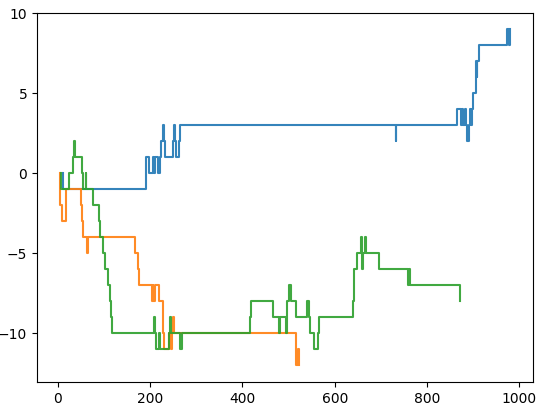
\includegraphics[scale=.5]{rwhw3-fig1.png}

Then I generated a a plot comparing the ensemble mean squared displacement(blue) and the temporal mean squared displacement of three realizations(red orange and green). I do not know why my plot for ensemble average has a spike at the start. But the rest of the graph does seem to follow a $t^{1/2}$ scaling.

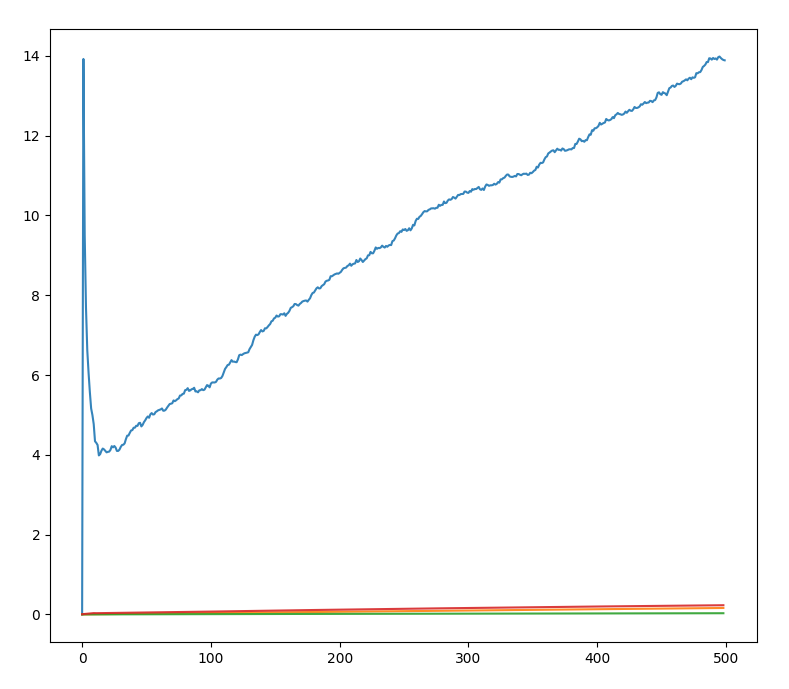
\includegraphics[scale=.6]{rwhw3-fig2.png}

Next we will look at the diffusion coefficients of the temporal MSDs. We created a probability density plot of the diffusion coefficients 

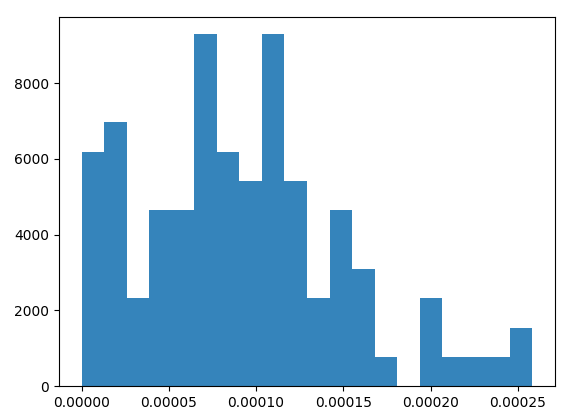
\includegraphics[scale=.5]{rwhw3-fig3.png}

Finally we will look at how the temporal MSD changes(which is proportional to the diffusion coefficient) with the time interval of each realization. So we will plot the a graph comparing the log of the time intervals(on the $x$-axis) with the log of the diffusion coefficients ($y$-axis).

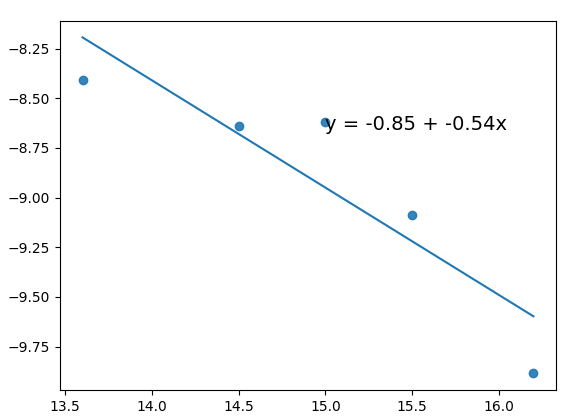
\includegraphics[scale=.5]{rwhw3-fig4.png}

We can see that the slope is roughly $-.5$ which agrees with the paper and theoretical expectations.\\


\item[(7)]
The pdf of $X$ is $p(x)=\frac{b}{\pi(x^2+b^2)}$ and let the CDF be $F(x)$.
Now let $Z=X^2$ and consider the CDF of $Z$, that is $F_Z(z)=P[Z\leq z]=P[X^2\leq z]=P[-\sqrt{z}\leq X\leq \sqrt{z}]$. And using the CDF of $X$ we therefore know that $F_Z(z)=F(\sqrt{z})-F(-\sqrt{z})$. And so the PDF of $Z$ is therefore 
$$p(z)=\frac{d}{dz}\int_{-\sqrt{z}}^{\sqrt{z}}p(x)dx= 2\frac{d}{dz}\int_{0}^{\sqrt{z}}p(x)dx=2p(\sqrt{z})\cdot \frac{1}{2\sqrt{z}}$$
So we know that the PDF of $Z$ is $$p(z)=\frac{b}{\pi\left(b^{2}+z\right)\sqrt{z}}$$
% https://anilbs.me/generation-of-power-law-samples-with-inverse-transform-sampling-python-r-and-julia/
\end{itemize}

\newpage
\section*{Appendix}
\lstinputlisting[language=Python]{rw-hw3.py}
%I did not have time to modify my code to make it faster using array operations.\\
%Problem 4
%\lstinputlisting[language=Python]{rw-hw2.py}
%Problem 5
%\lstinputlisting[language=Python]{rw-hw2-p5.py}


\end{document}


